\documentclass[tikz]{standalone}

  \begin{document}
  \begin{figure}
  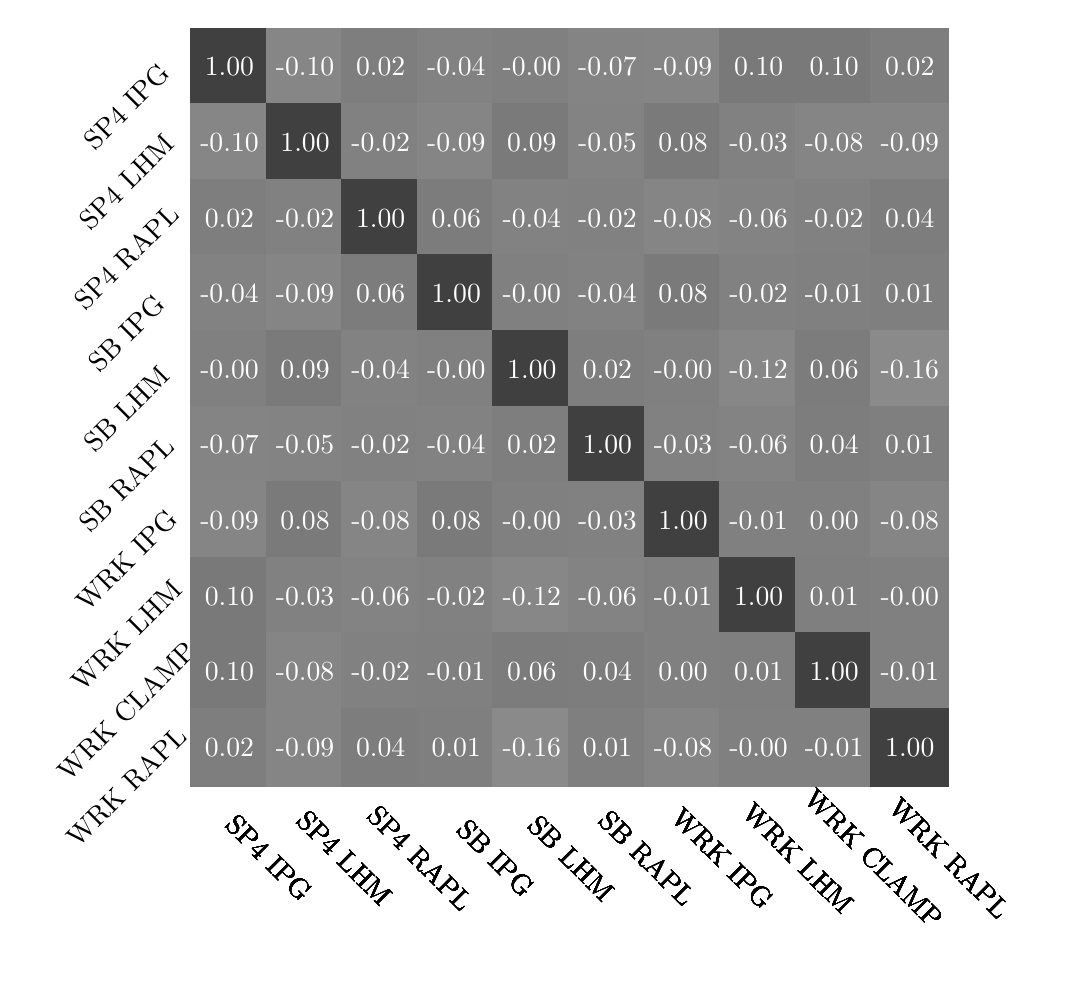
\begin{tikzpicture}[scale=0.6]
    \foreach \y [count=\n] in {{1.00, -0.10, 0.02, -0.04, -0.00, -0.07, -0.09, 0.10, 0.10, 0.02},{-0.10, 1.00, -0.02, -0.09, 0.09, -0.05, 0.08, -0.03, -0.08, -0.09},{0.02, -0.02, 1.00, 0.06, -0.04, -0.02, -0.08, -0.06, -0.02, 0.04},{-0.04, -0.09, 0.06, 1.00, -0.00, -0.04, 0.08, -0.02, -0.01, 0.01},{-0.00, 0.09, -0.04, -0.00, 1.00, 0.02, -0.00, -0.12, 0.06, -0.16},{-0.07, -0.05, -0.02, -0.04, 0.02, 1.00, -0.03, -0.06, 0.04, 0.01},{-0.09, 0.08, -0.08, 0.08, -0.00, -0.03, 1.00, -0.01, 0.00, -0.08},{0.10, -0.03, -0.06, -0.02, -0.12, -0.06, -0.01, 1.00, 0.01, -0.00},{0.10, -0.08, -0.02, -0.01, 0.06, 0.04, 0.00, 0.01, 1.00, -0.01},{0.02, -0.09, 0.04, 0.01, -0.16, 0.01, -0.08, -0.00, -0.01, 1.00},} {
    % column labels
    \foreach \a [count=\n] in {SP4 IPG,SP4 LHM,SP4 RAPL,SB IPG,SB LHM,SB RAPL,WRK IPG,WRK LHM,WRK CLAMP,WRK RAPL} {
      \node[minimum size=10mm, xshift=0.5cm, rotate=-45] at (\n*1.6, -18.35) {\a};
    }
    % heatmap tiles
    \foreach \x [count=\m] in \y {
      \pgfmathsetmacro{\xa }{(\x + 1) / 2 * 100}
      \node[fill=darkgray!\xa!lightgray, minimum size=10mm, text=white, font={\normalsize}] at (\m*1.6,-\n*1.6) {\x};
    }
  }
    % row labels
    \foreach \a [count=\i] in {SP4 IPG,SP4 LHM,SP4 RAPL,SB IPG,SB LHM,SB RAPL,WRK IPG,WRK LHM,WRK CLAMP,WRK RAPL} {
      \node[minimum size=10mm, xshift=-0.35cm, yshift=-0.5cm, rotate=45] at (0,-\i*1.6) {\a};
    }
  \end{tikzpicture}
  \caption{This is a test}
  \label{tab:BinaryTrees}
  \end{figure}
  \end{document}